\documentclass[12pt]{amsart}
\usepackage[T1]{fontenc}
\usepackage[utf8]{inputenc}

\usepackage[top=1.95cm, bottom=1.95cm, left=2.35cm, right=2.35cm]{geometry}

\usepackage{amsmath}
\usepackage{amssymb}
\usepackage{enumitem}
\usepackage{multicol}
\usepackage[french]{babel}
\usepackage[
    type={CC},
    modifier={by-nc-sa},
	version={4.0},
]{doclicense}

\usepackage{lymath}

\DeclareMathOperator{\taille}{\tau}

\newtheorem{fact}{Fait}
\newtheorem*{proof*}{Preuve}

\setlength\parindent{0pt}


\newcommand\squote[1]{\og #1 \fg{}}


\begin{document}

\title{BROUILLON - Faire des produits sur une hyperbole}
\author{Christophe BAL}
\date{22 Juillet 2019}
\maketitle


\begin{center}
	\hrule\vspace{.3em}
	{
		\fontsize{1.35em}{1em}\selectfont
		\textbf{Mentions \og légales \fg}
	}
			
	\vspace{0.45em}
	\doclicenseThis
	\hrule
\end{center}



\setcounter{tocdepth}{2}
\tableofcontents




\section{\texorpdfstring{Comment additionner des nombres grâce à l'hyperbole d'équation $y = \frac{1}{x}$}%
                        {Comment additionner des nombres grâce à l'hyperbole d'équation y = 1/x}}

Dans un repère orthogonal, donnons nous l'hyperbole $\geoset{H} : y = \frac{1}{x}$ . Plaçons-y les points $A$ , $B$ et $P$ d'abscisses respectives $a$ , $b$ et  $p = ab$ .
Observez
\footnote{
	Pour conjecturer plus facilement quelque chose, utilisez le fichier GeoGebra \texttt{base-tool.ggb} manipulable dynamiquement qui est disponible sur le lieu de téléchargement de ce document.
}
les trois cas ci-dessous et essayez de conjecturer quelque chose \emph{(la réponse est donnée dans la page suivante)}
\footnote{
	On sait \emph{\og additionner \fg} sur un cercle et sur $\geoset{P} : y = x^2$ .
	Or $yx$ , $x^2 - y^2$ et $x^2 - y$ sont des formes quadratiques qui ont des propriétés gémétriques communes.
	Avec tout ceci en tête, la recherche proposée ici devient des plus naturelles.
}.


\begin{center}
	\footnotesize
	\itshape

	\fbox{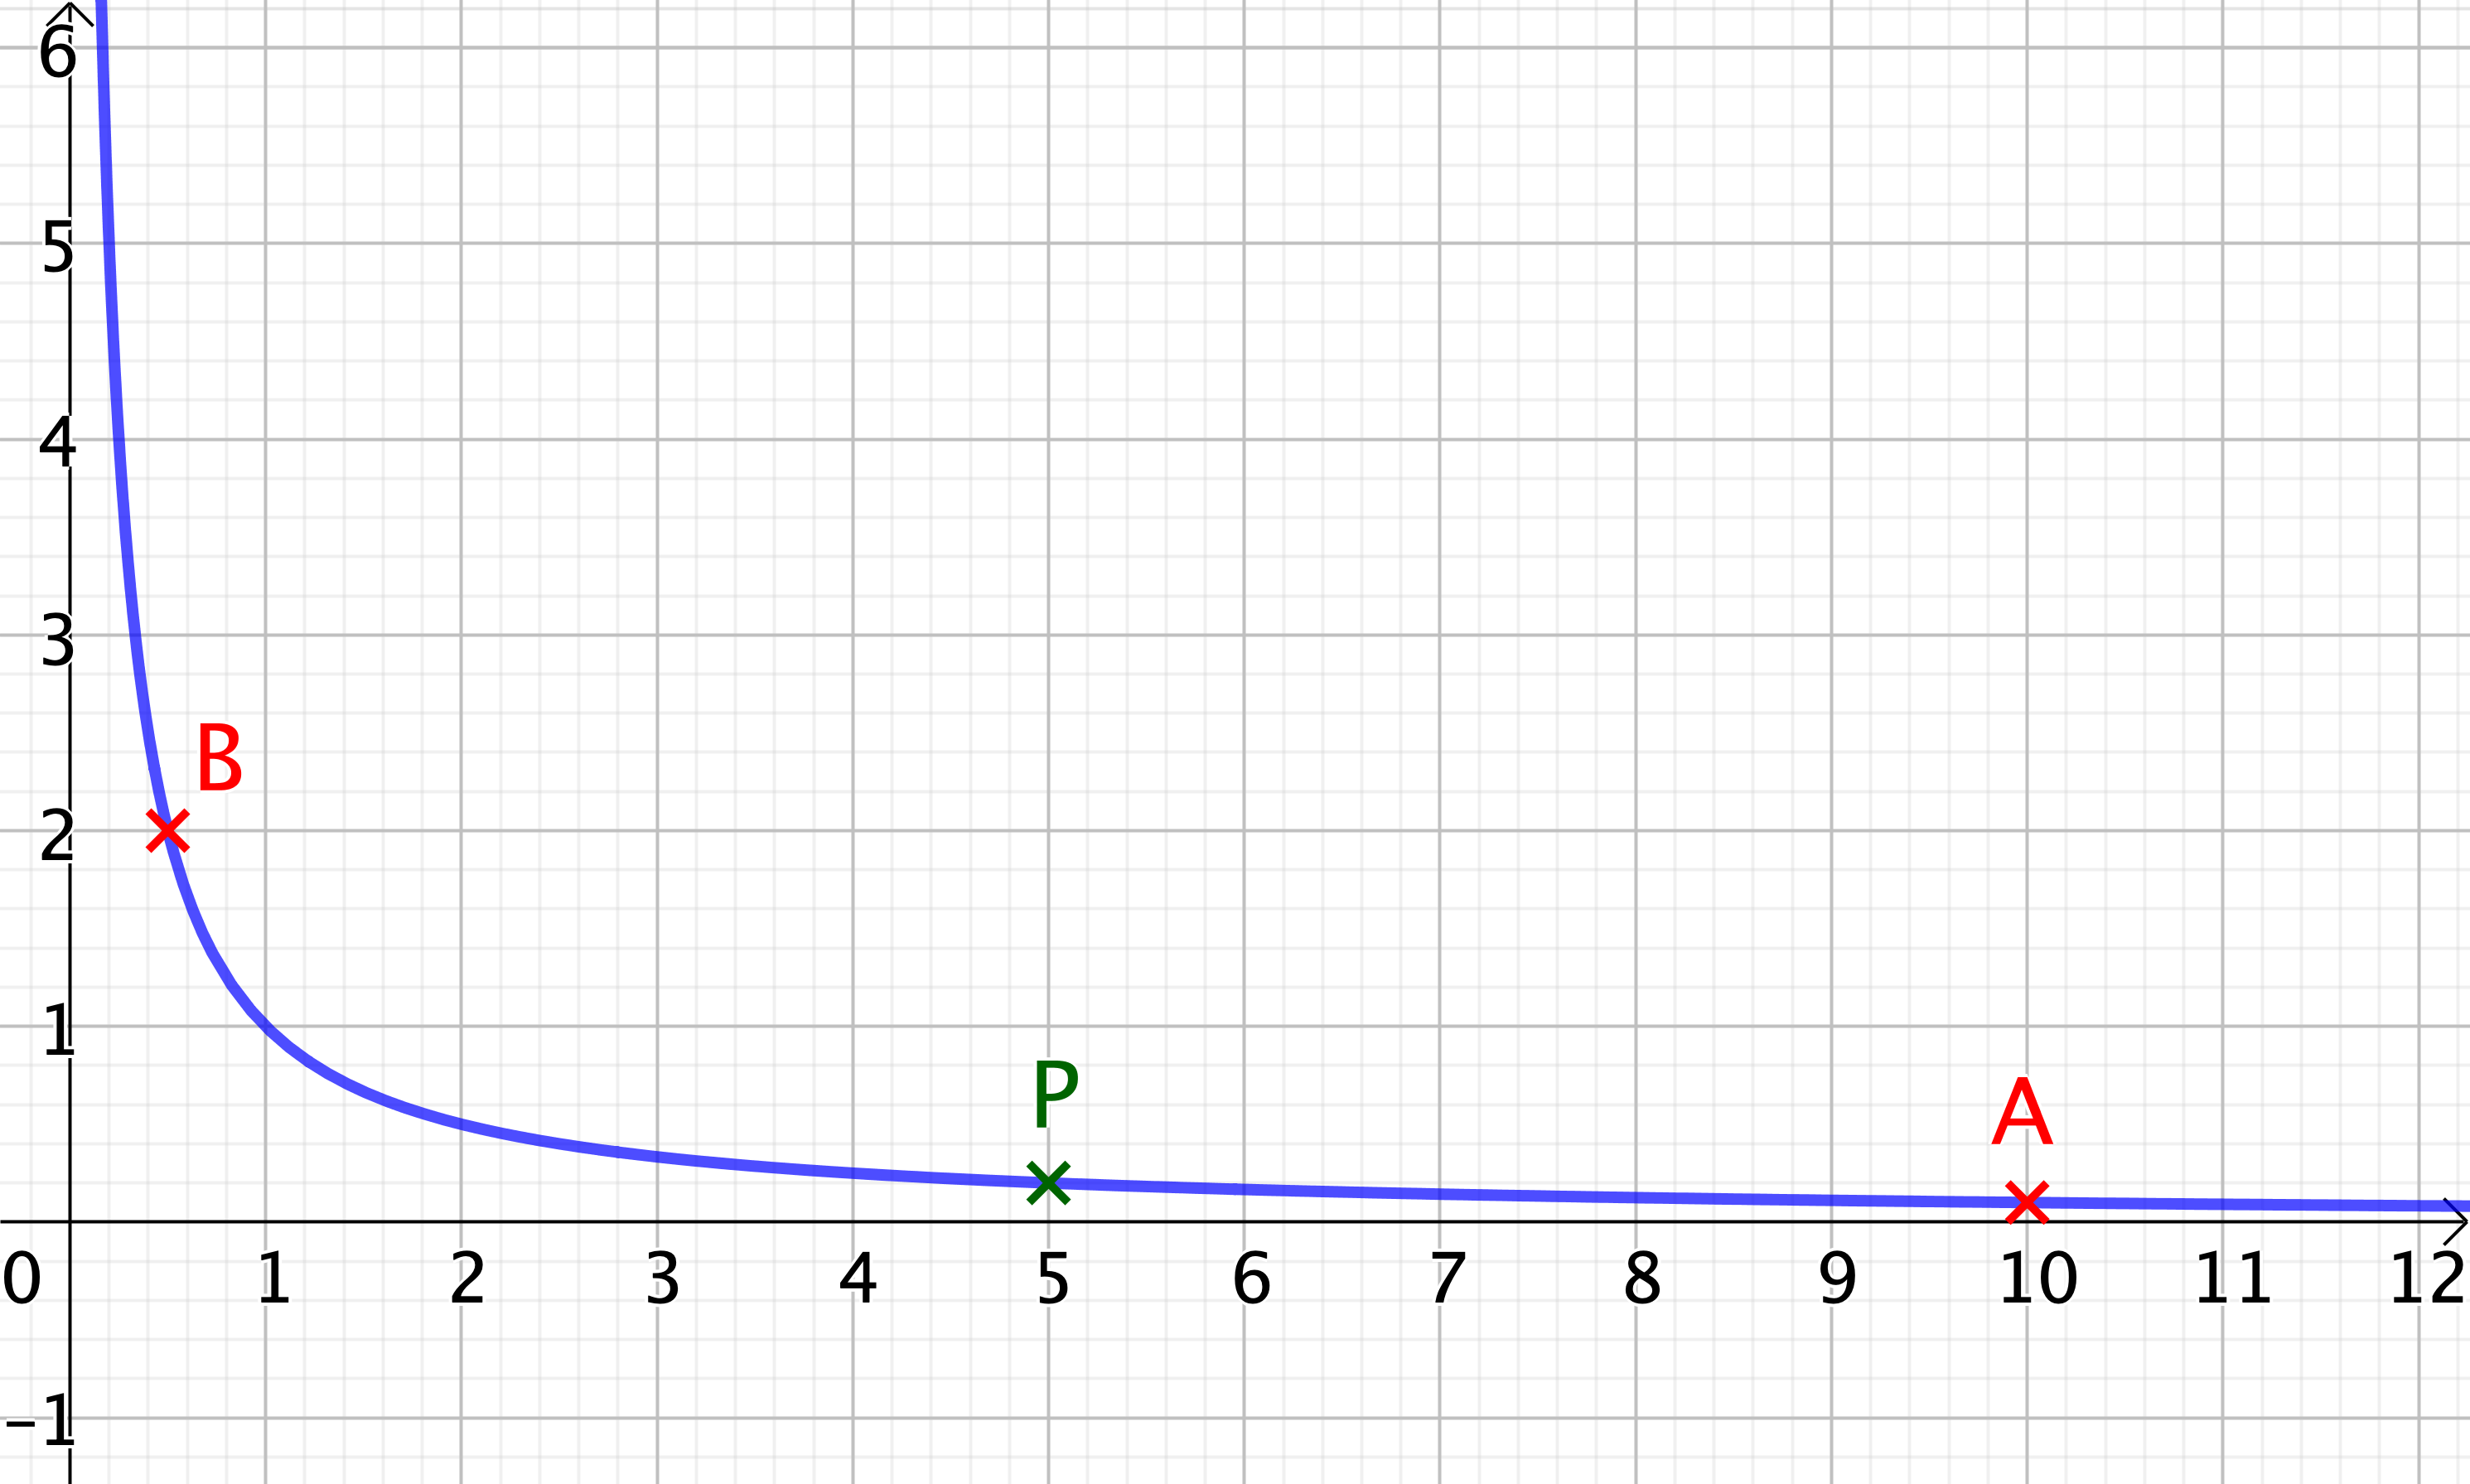
\includegraphics[scale = .75]{product-on-hyperbolas/conjecture/a-and-b-positive.png}}
	
	\smallskip
	Cas où $a > 0$ et $b > 0$

	\medskip
	
	\fbox{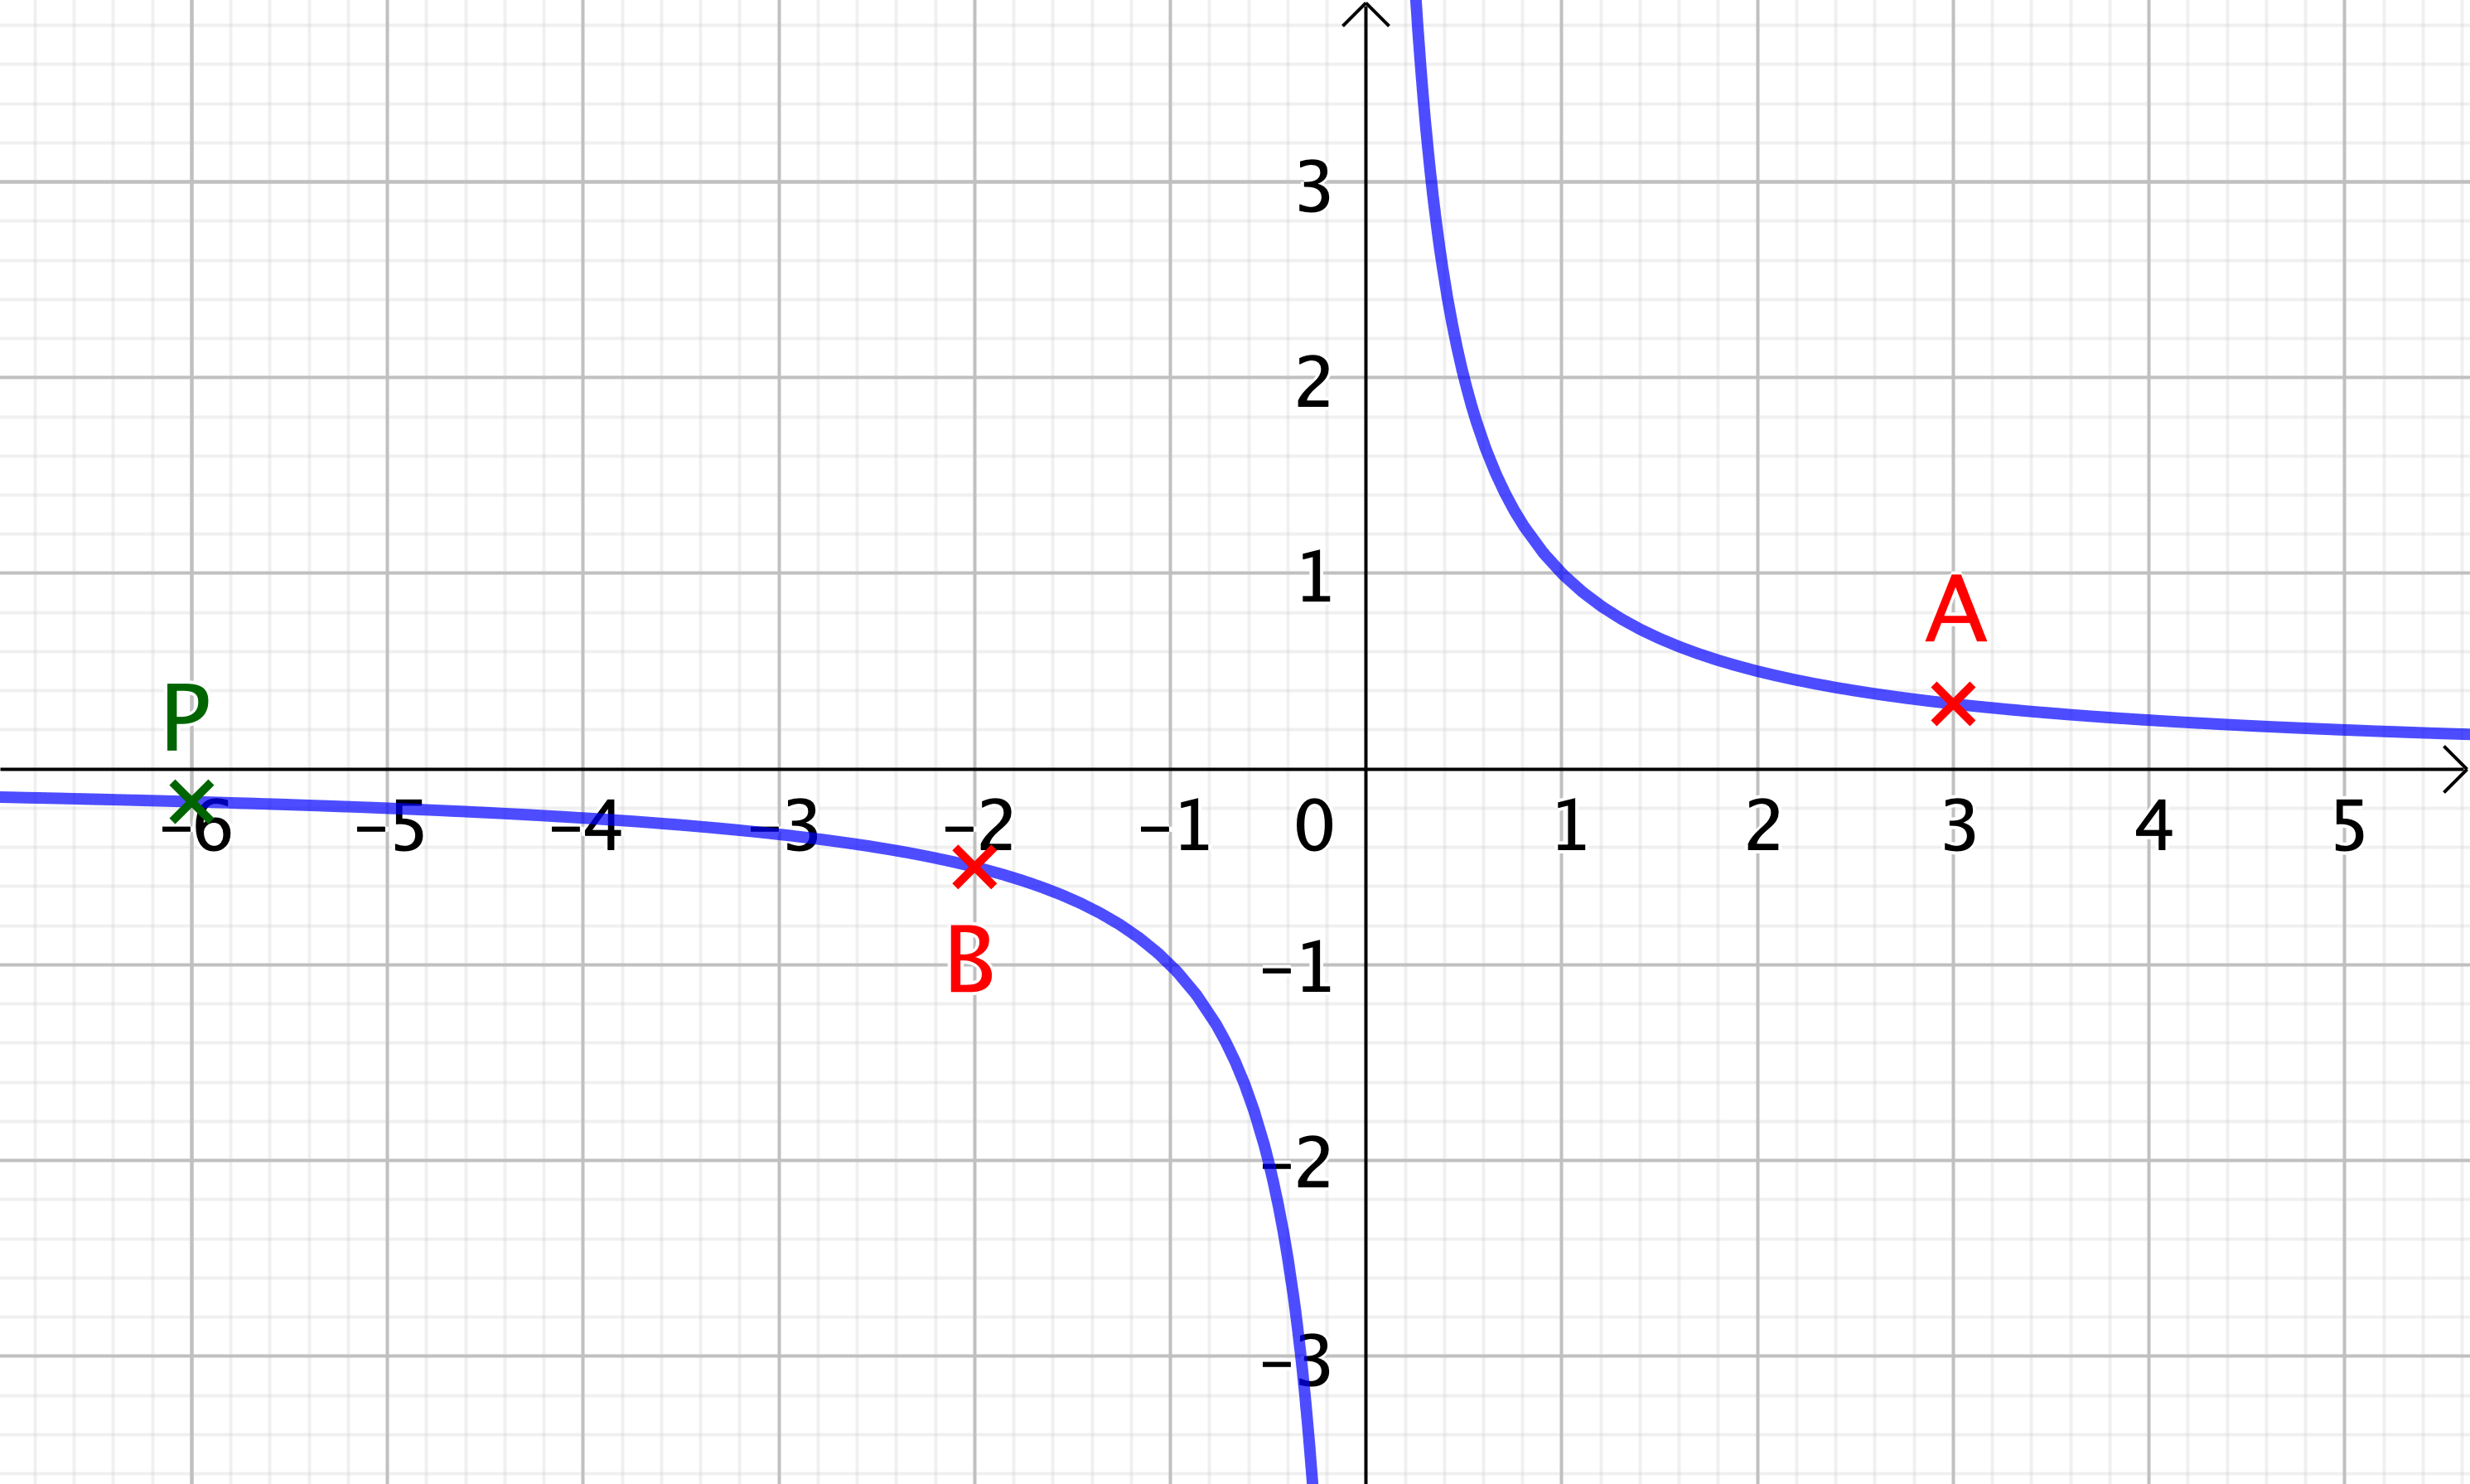
\includegraphics[scale = .75]{product-on-hyperbolas/conjecture/a-and-b-diff-signs.png}}
	
	\smallskip
	Cas où $a < 0$ et $b > 0$

	\medskip

	\fbox{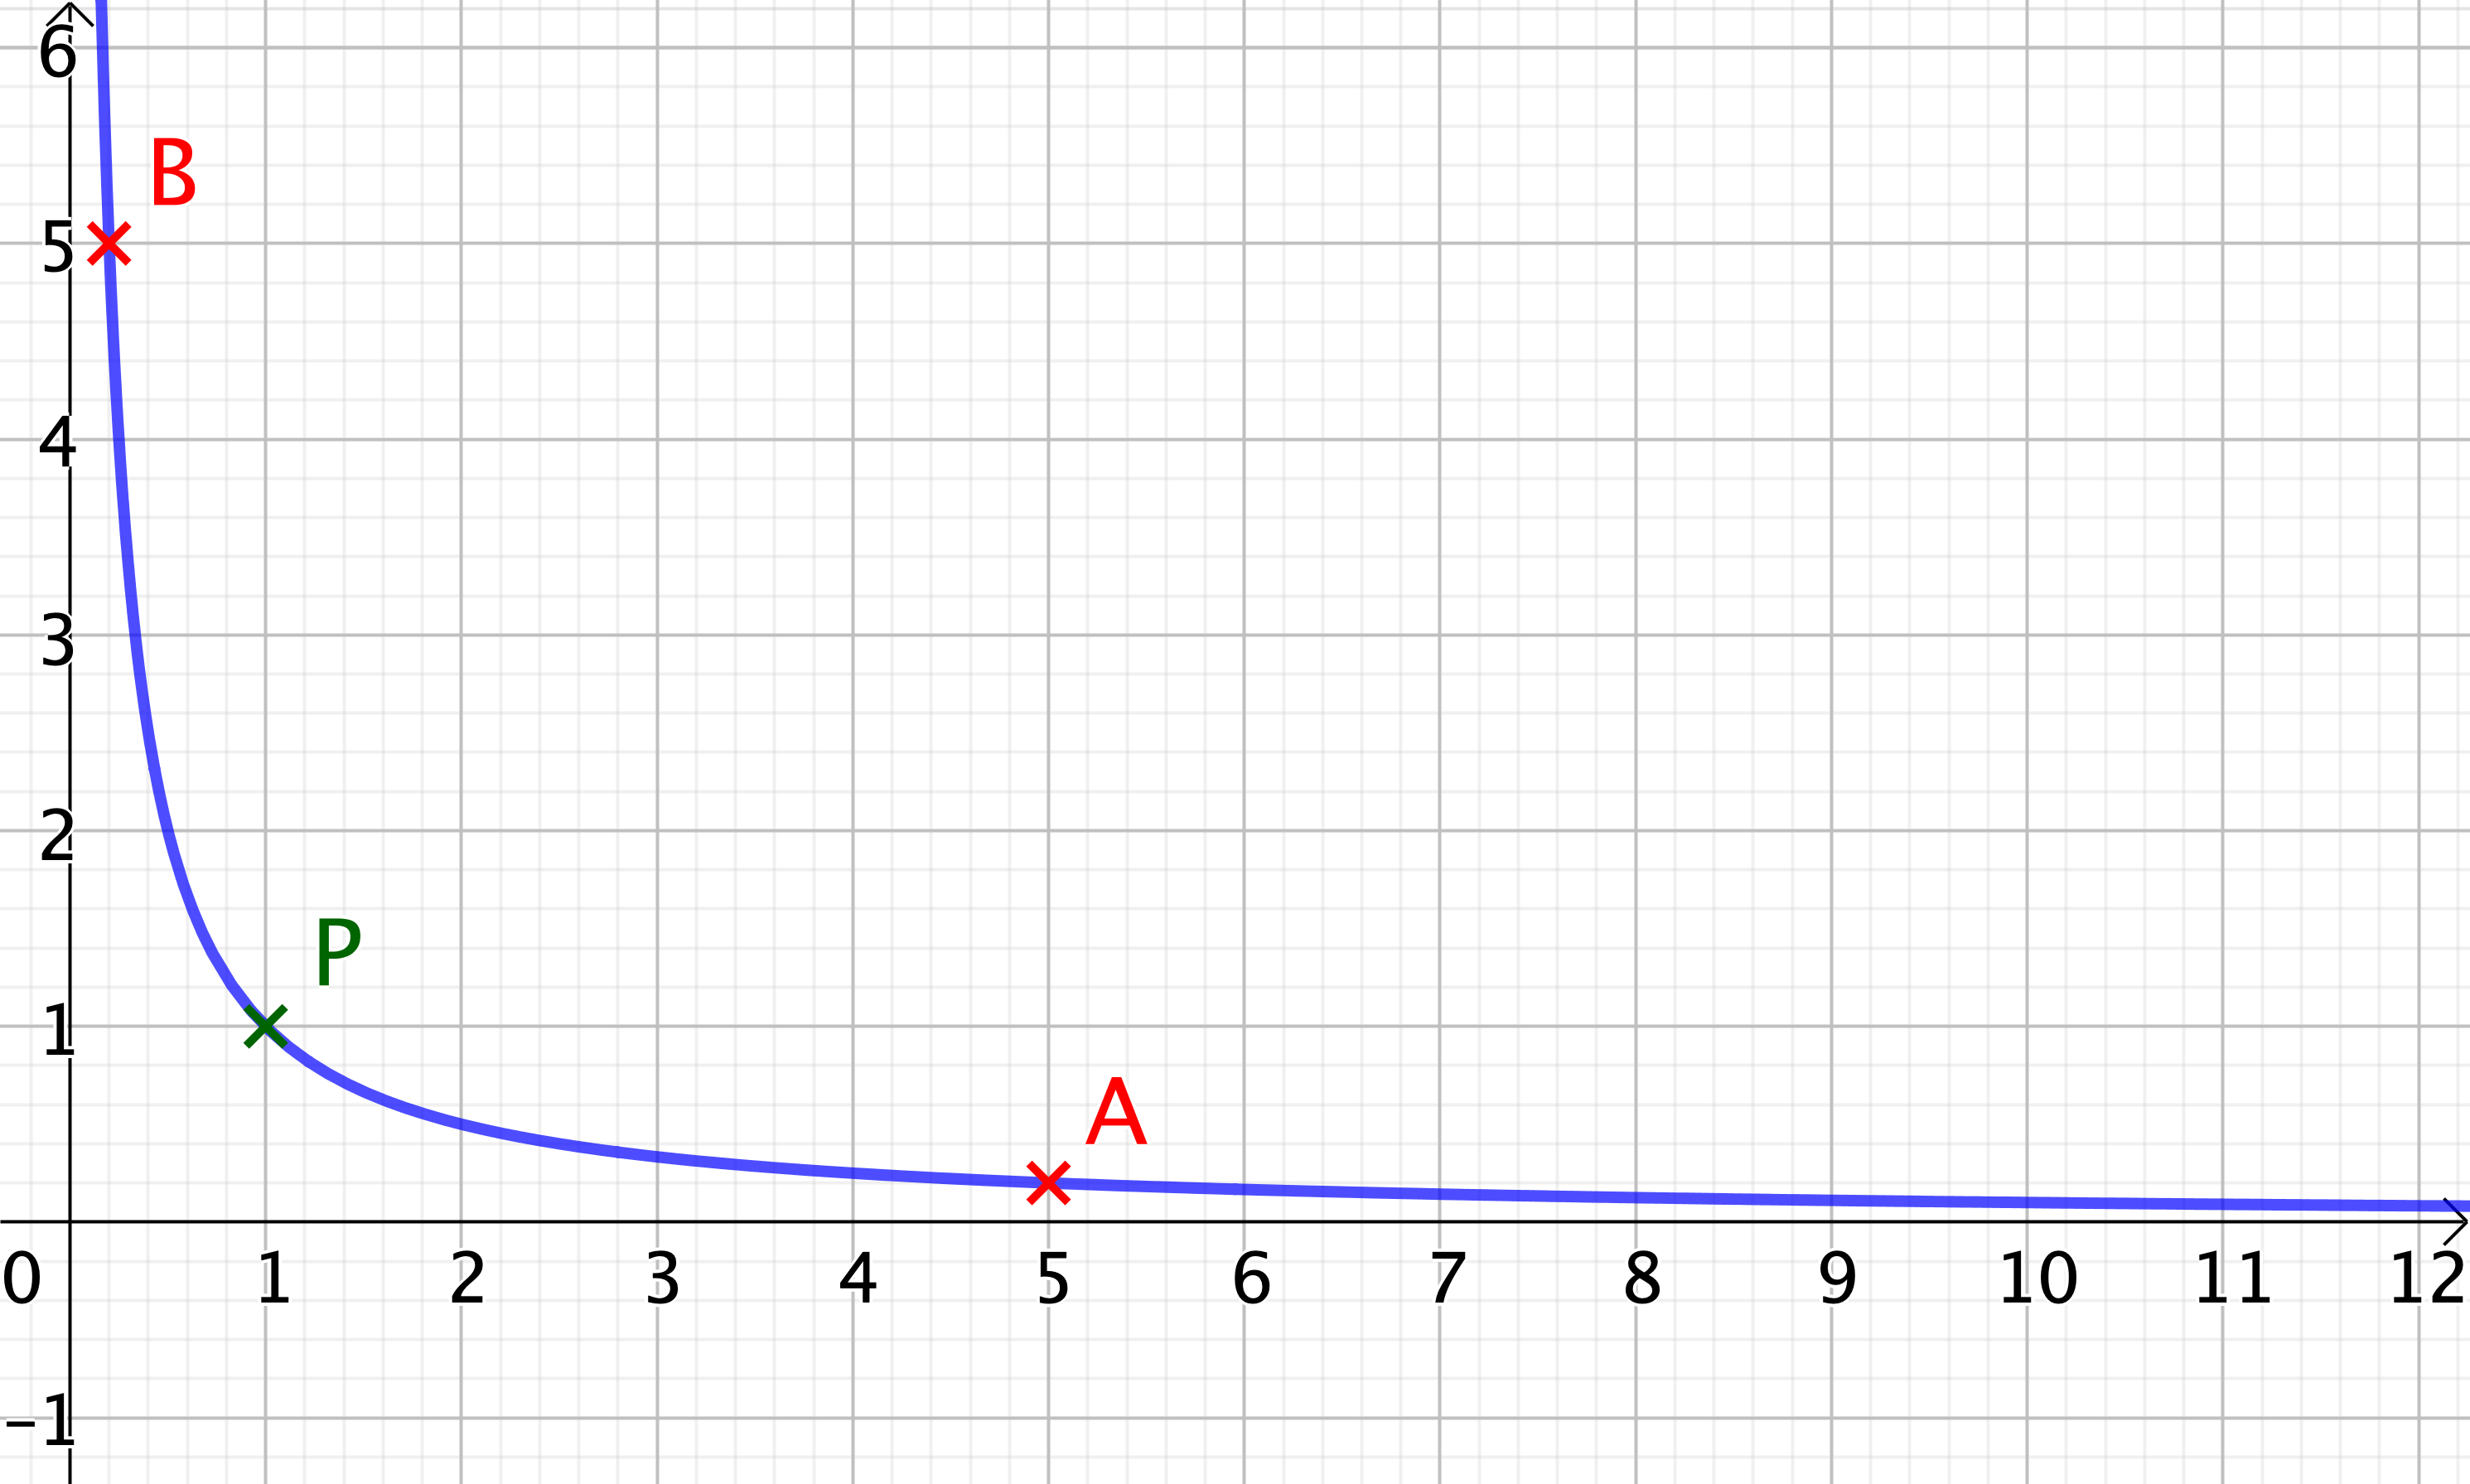
\includegraphics[scale = .75]{product-on-hyperbolas/conjecture/a-and-b-inverse.png}}
	
	\smallskip
	Cas où $a b = 1$
\end{center}


\newpage

Pour mieux voir ce qu'il se passe, ajoutons $E(1 ; 1)$ , ce qui semble naturel car $1$ est le neutre de la multiplication, et traçons quelques droites. Voici ce que cela donne.

\begin{center}
	\footnotesize
	\itshape

	\fbox{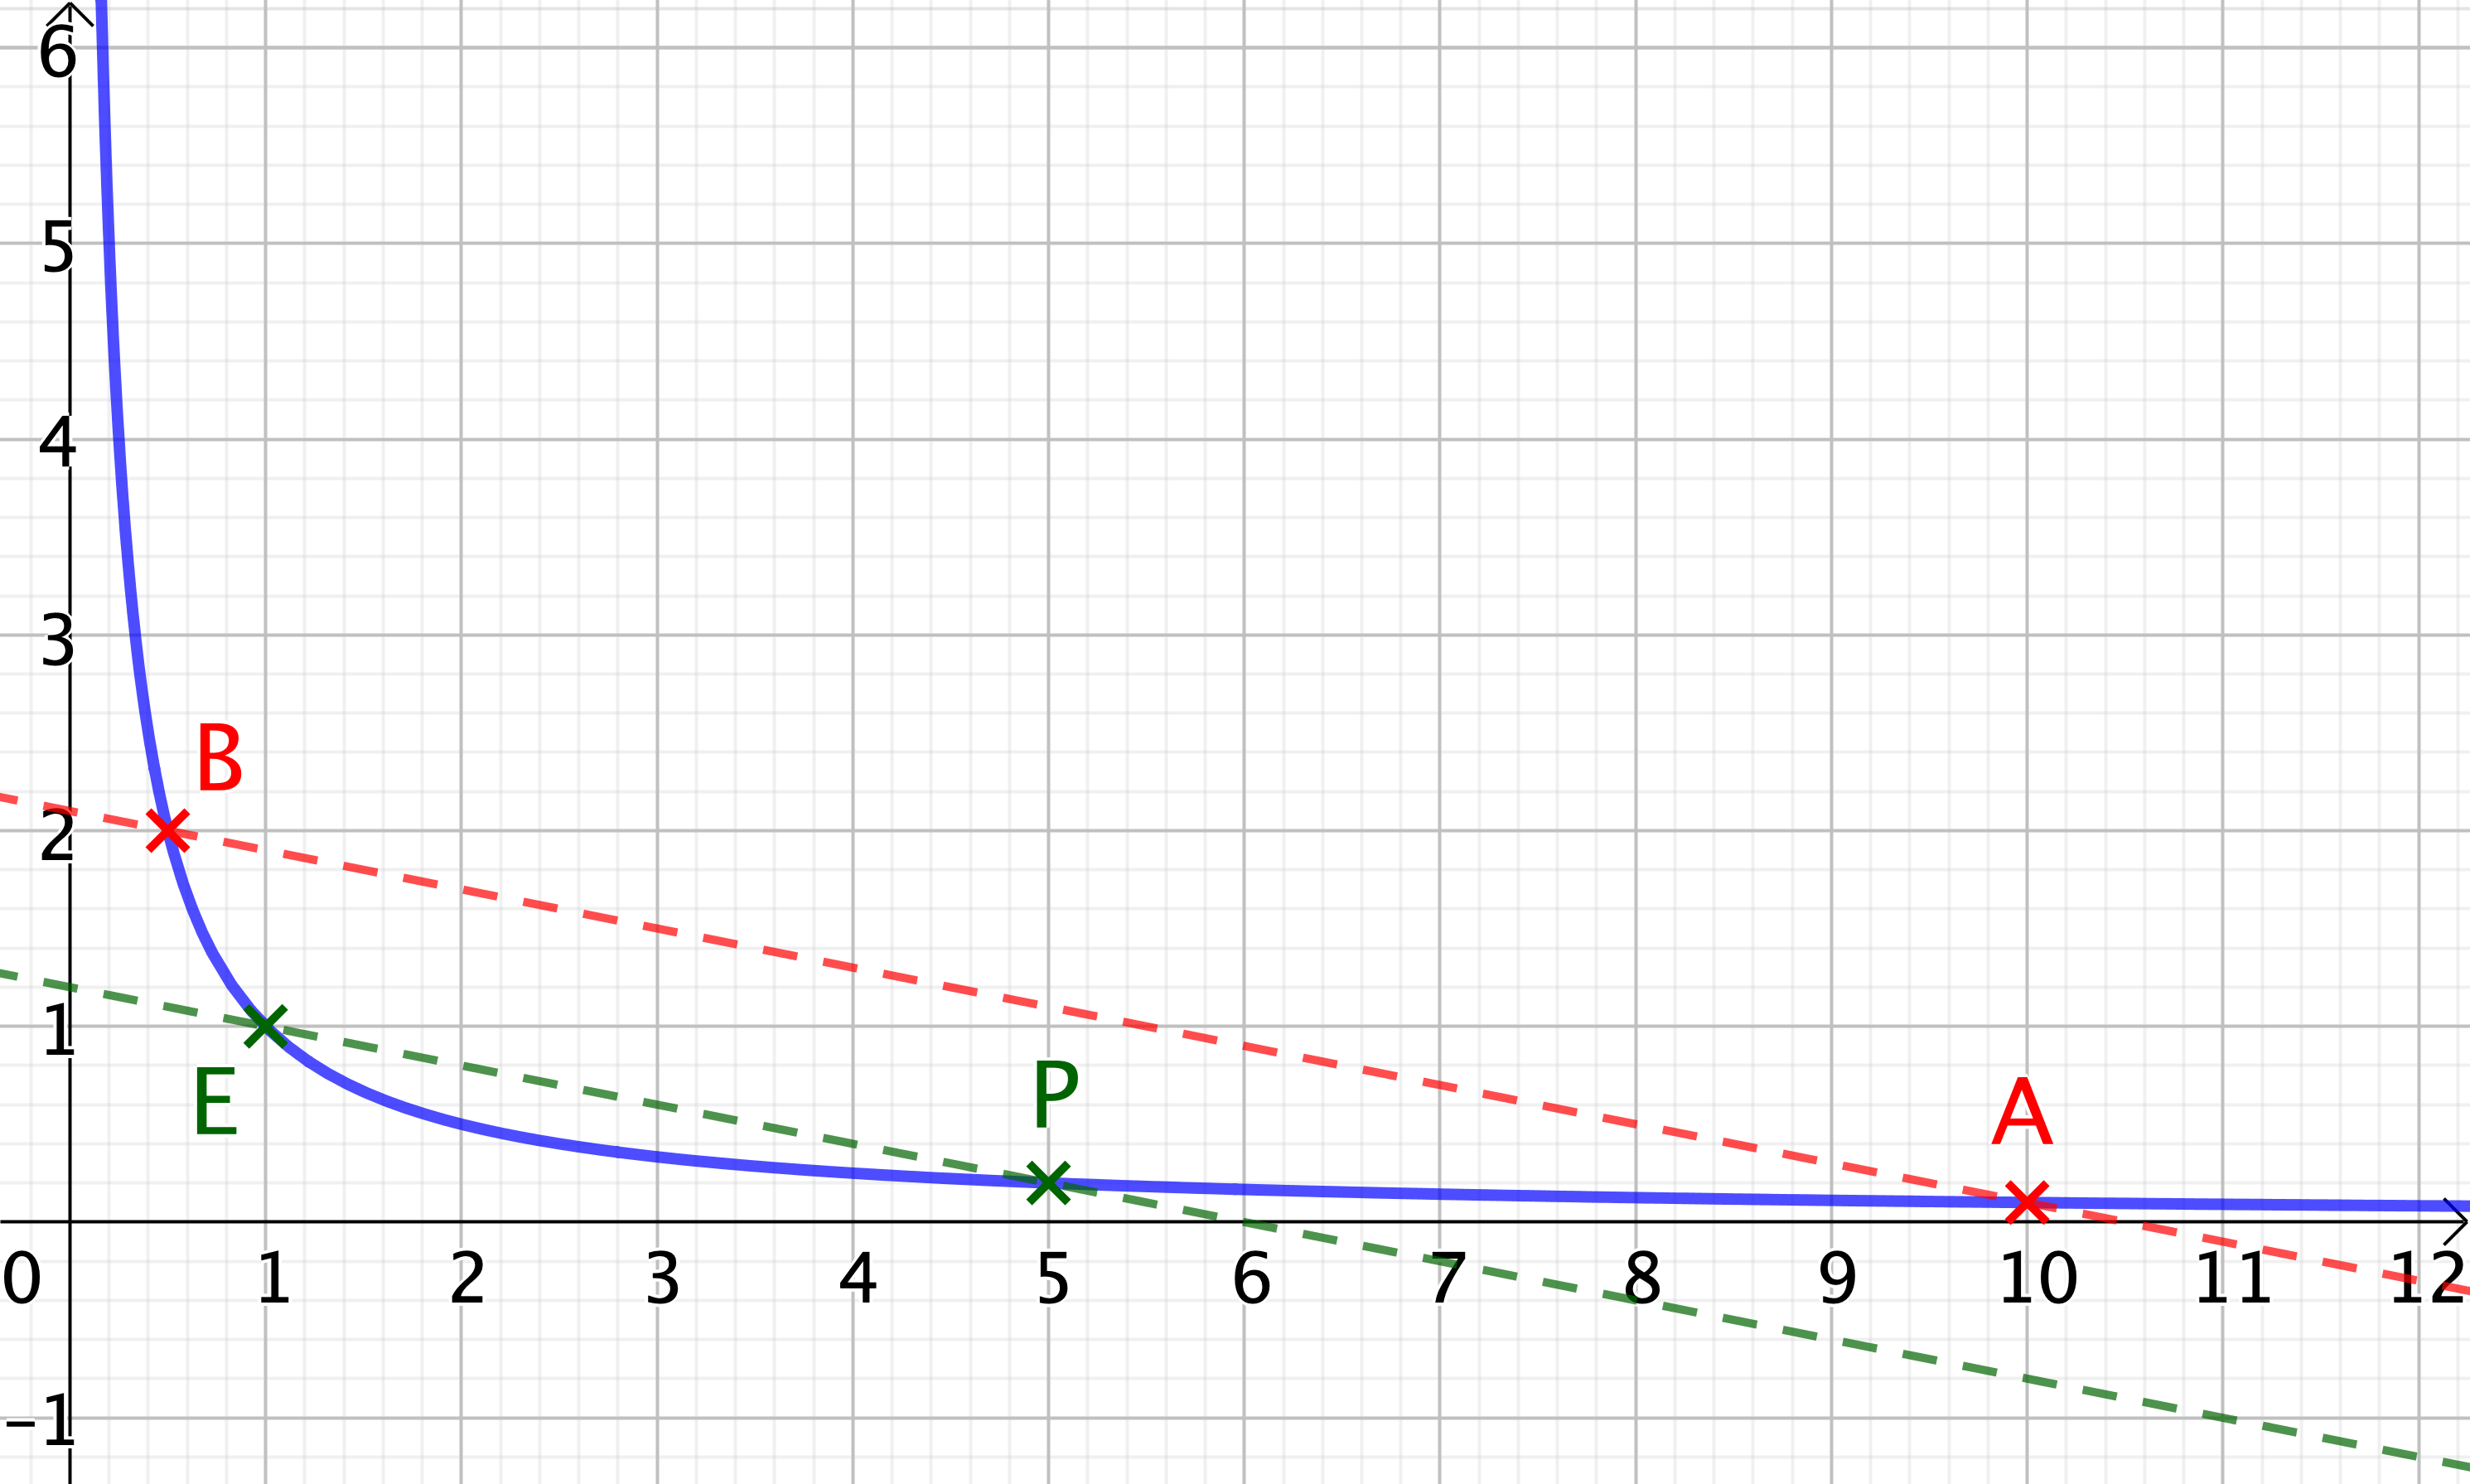
\includegraphics[scale = .75]{product-on-hyperbolas/conjecture/a-and-b-positive-with-lines.png}}
	
	\smallskip
	Cas où $a > 0$ et $b > 0$

	\medskip

	\fbox{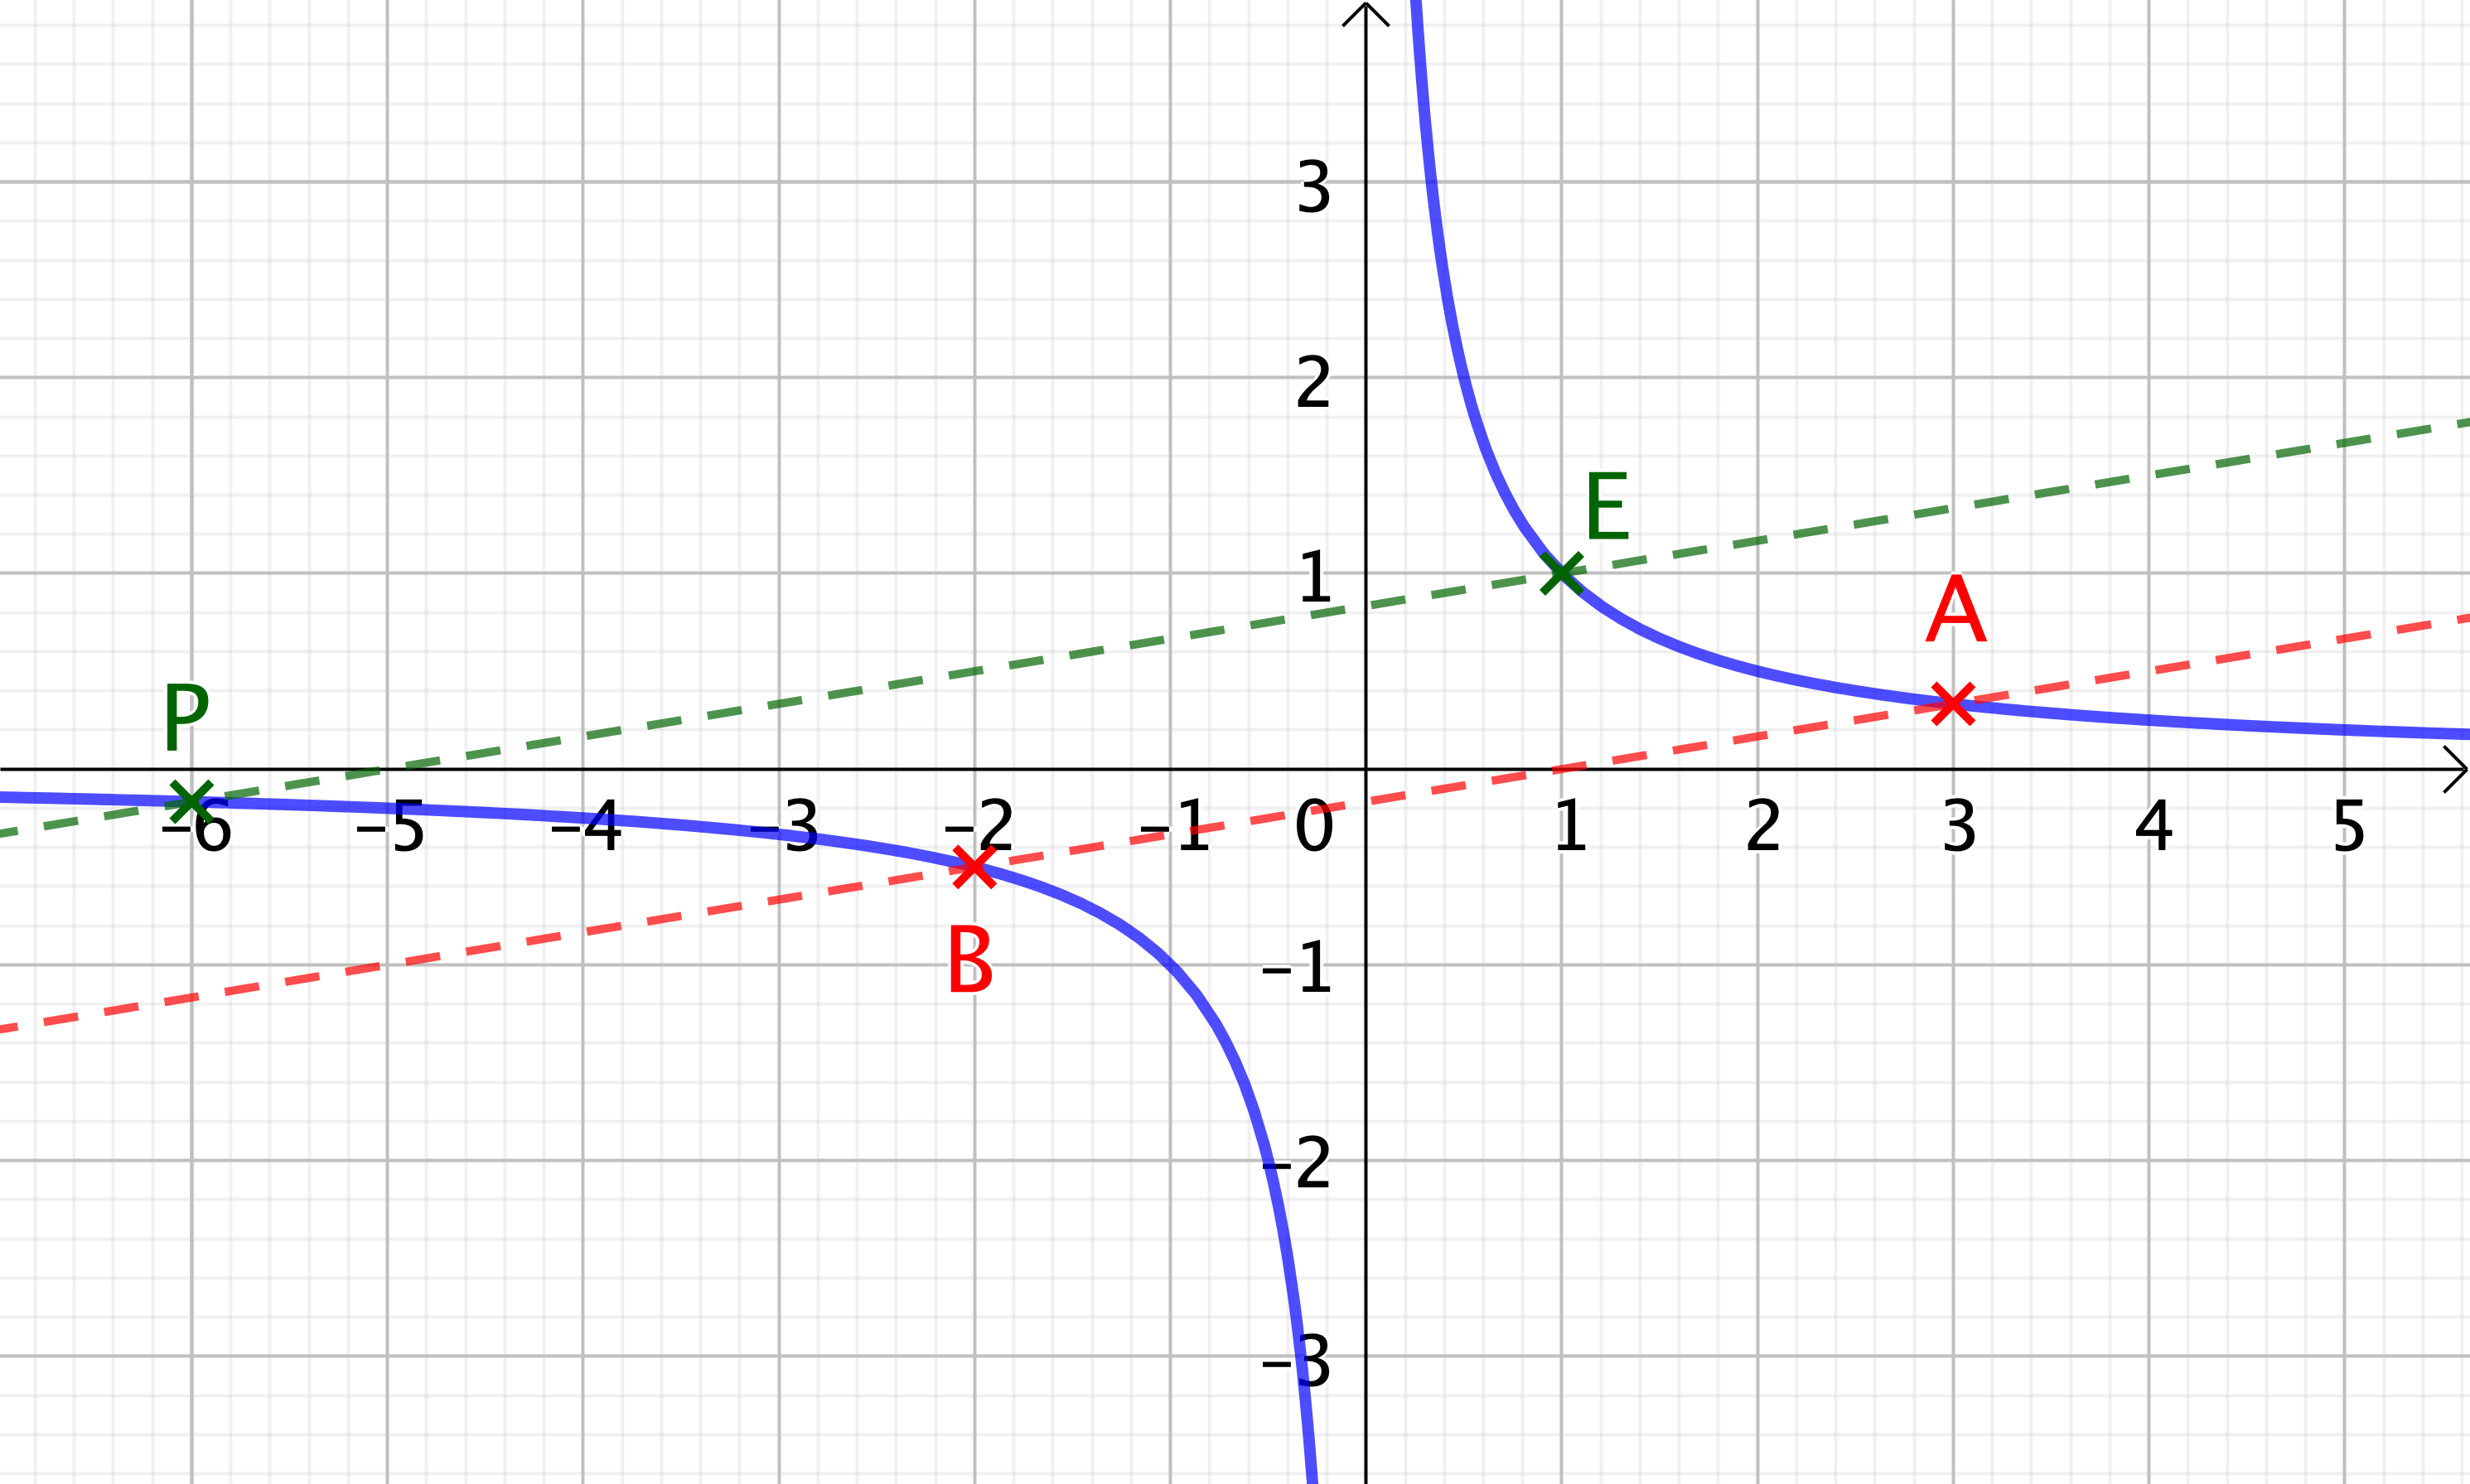
\includegraphics[scale = .75]{product-on-hyperbolas/conjecture/a-and-b-diff-signs-with-lines.png}}
	
	\smallskip
	Cas où $a < 0$ et $b > 0$

	\medskip

	\fbox{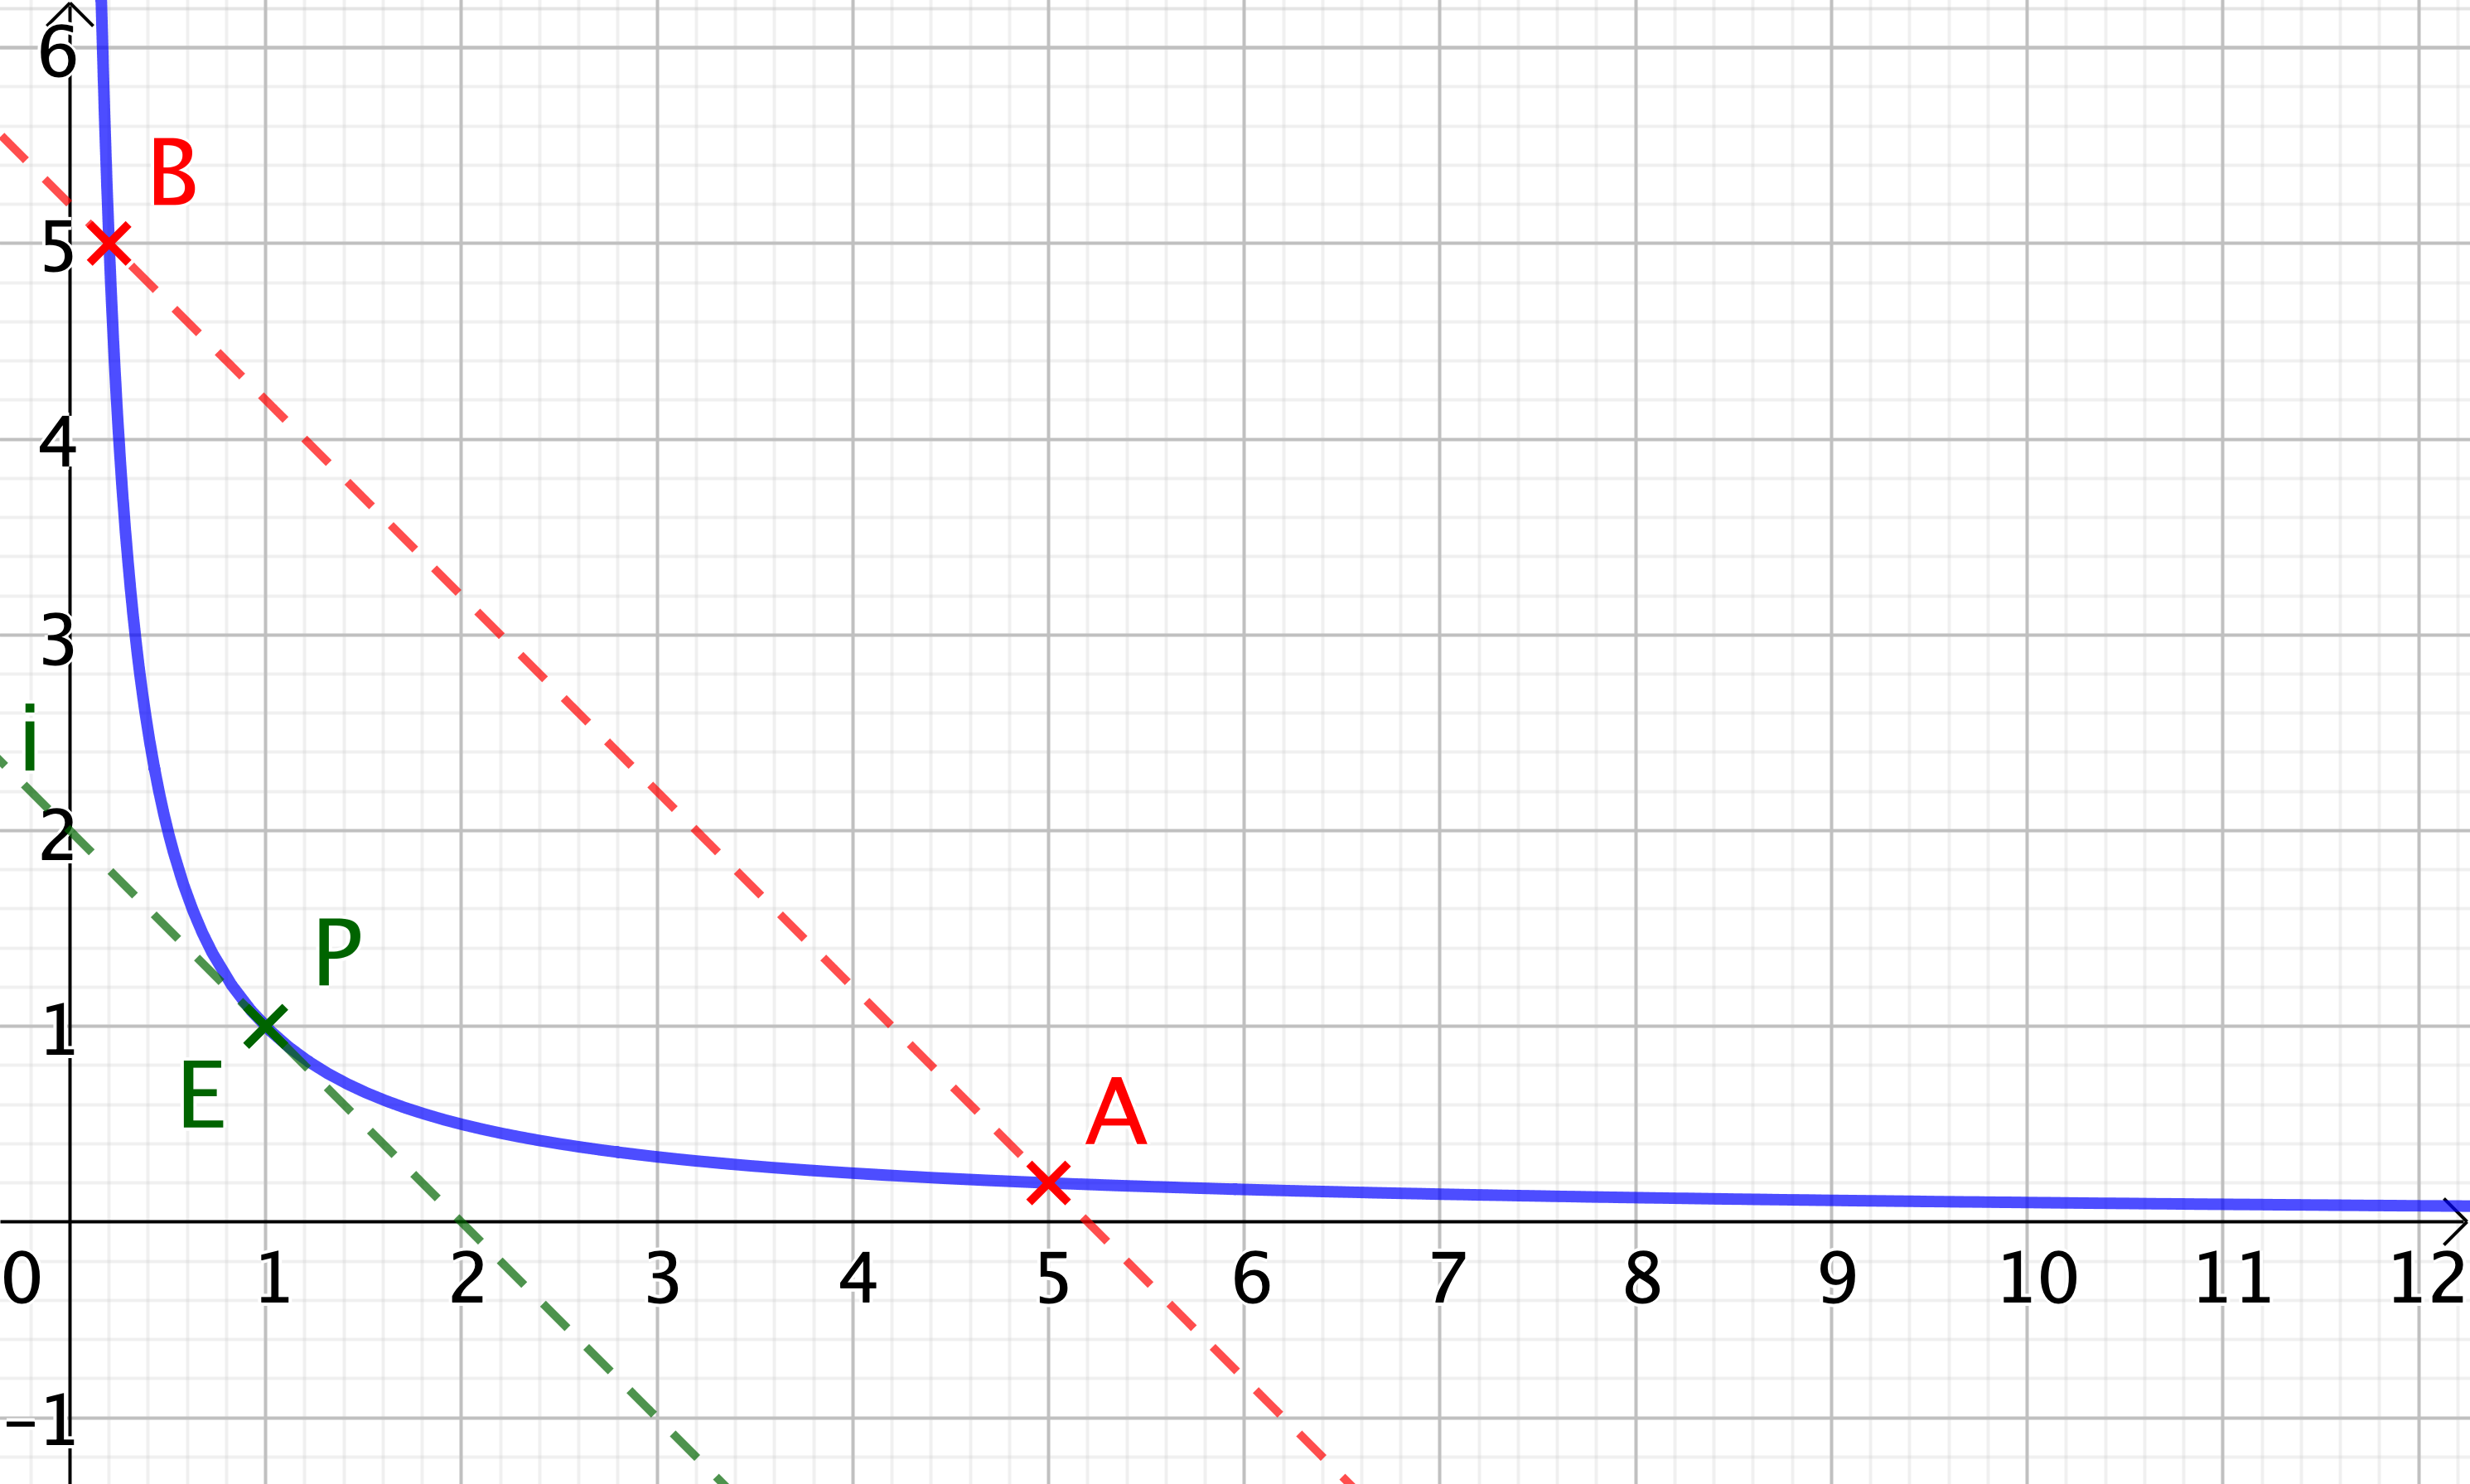
\includegraphics[scale = .75]{product-on-hyperbolas/conjecture/a-and-b-inverse-with-lines.png}}
	
	\smallskip
	Cas où $a b = 1$
\end{center}


\medskip

Il devient évident de conjecturer que le point $P$ se construit géométriquement comme suit.

\begin{enumerate}
	\item \label{point-1} Si $x_A x_B \neq 1$ et $A \neq B$ alors on construit la parallèle à $(AB)$ passant par $E$ . Le point $P$ est le second point d'intersection de cette parallèle avec $\geoset{H}$  \emph{(notons qu'une droite coupe $\geoset{H}$ en au plus deux points)}.

	\item Si $x_A x_B = 1$ alors $P = E$ . Notons au passage que l'on peut voir ceci comme un cas limite du précédent avec un point d'intersection \squote{double}.

	\item Si $x_A x_B \neq 1$ et $A = B$ , on procède comme au point (\ref{point-1}) mais avec la parallèle à la tangente en $A$ à l'hyperbole $\geoset{H}$ .
\end{enumerate}


La section qui suit va valider cette conjecture qui donne un moyen très capillotracté de calculer un produit de deux réels non nuls via l'hyperbole $\geoset{H}$ .
Plus sérieusement, la construction ci-dessus est une propriété géométrique très jolie de l'hyperbole $\geoset{H}$ .




\section{Preuve de la validité de la conjecture} \label{proof}

\textbf{Cas 1.} \emph{Supposons que $x_A \neq \pm \, x_B$ de sorte que $x_S \neq 0$ .}

\medskip

La droite $(AB)$ a pour pente
$\frac{y_A - y_B}{x_A - x_B} = \frac{a^2 - b^2}{a - b} = a + b$ .
De plus, la droite $(OS)$ qui passe par l'origine $O$ du repère a pour pente
$\frac{y_S}{x_S} = \frac{x_S^2}{x_S} = x_S = a + b$ .
Les droites $(AB)$ et $(OS)$ sont bien parallèles comme nous l'avons affirmé.


\bigskip

\textbf{Cas 2.} \emph{Supposons que $x_A = - x_B$ .}

\medskip

Comme $x_S = a + b = 0$ , nous avons bien $S = O$ .


\bigskip

\textbf{Cas 3.} \emph{Supposons que $x_A = x_B \neq 0$ .}

\medskip

Dans ce cas, $x_S = 2a \neq 0$ donc la droite $(OS)$ a pour pente
$x_S = 2a$ qui est bien la pente de la tangente en $A$ à la parabole $\geoset{P}$ .



\section{\texorpdfstring{Toute hyoerbole d'équation $y = \frac{a x + b}{c x + d}$ a une structure de groupe}%
                        {Toute hyoerbole d'équation y = (a x + b) / (c x + d) a une structure de groupe}}
      
Le procédé de construction que nous venons de prouver se \emph{\og conserve \fg} par translations, et aussi par dilatations verticales et horizontales.
Il se trouve que ce sont ces transformations qui permettent d'obtenir une hyperbole $\geoset{H}\,^\prime : y = \frac{a x + b}{c x + d}$ , où $c \neq 0$ et $ad - bc \neq 0$ 
\footnote{
	La condition $ad - bc \neq 0$ évite d'avoir une simplification de $\frac{a x + b}{c x + d}$ en une fonction affine comme on peut le constater en considérant les vecteurs $\vect{u}(a ; b)$ et $\vect{v}(c ; d)$ , puis en notant que $ad - bc = \det \left( \vect{u} ; \vect{v} \right)$ .  
},
à partir de celle de l'hyperbole $\geoset{H} : y = \frac{1}{x}$ .
Nous pouvons donc munir toute hyperbole $\geoset{H}\,^\prime : y = \frac{a x + b}{c x + d}$ d'une structure de groupe isomorphe à celle de $(\RRs ; \times)$ , et ceci avec un procédé géométrique simple pour \emph{\og multiplier \fg} sur $\geoset{H}\,^\prime$ . Que c'est joli !


\end{document}
